\documentclass[10pt]{article}
\usepackage[margin=1in, paperwidth=8.5in, paperheight=11in]{geometry}
\usepackage{ifpdf,amsmath, amssymb, comment, color, graphicx, stmaryrd,setspace,enumitem,tikz, fancyhdr, wrapfig, textcomp, units, mathptmx, pdfpages, cancel, multicol}
\usepackage{hyperref}
\hypersetup{
    colorlinks=true,
    urlcolor=blue,
}

\setlength{\headheight}{14.5pt}
\newcommand{\Q}{\mathbb{Q}}
\newcommand{\R}{\mathbb{R}}
\newcommand{\Z}{\mathbb{Z}}
\newcommand{\vu}{\mathbf{u}}
\newcommand{\vv}{\mathbf{v}}
\newcommand{\vw}{\mathbf{w}}
\newcommand{\vi}{\mathbf{i}}
\newcommand{\vj}{\mathbf{j}}
\newcommand{\vk}{\mathbf{k}}
\newcommand{\vn}{\mathbf{n}}
\newcommand{\vr}{\mathbf{r}}
\newcommand{\va}{\mathbf{a}}
\newcommand{\vF}{\mathbf{F}}
\newcommand{\vL}{\mathbf{L}}
\newcommand{\vT}{\mathbf{T}}
\newcommand{\vN}{\mathbf{N}}
\newcommand{\proj}{\operatorname{proj}}
\newcommand{\orth}{\operatorname{orth}}
\newcommand\del\nabla
\newcommand\dotp[1][.5]{\,\mathbin{\vcenter{\hbox{\scalebox{#1}{$\bullet$}}}}\,}

% Solution text is in red. If you want the solutions to show, remove the \iffalse from the definition of the \red command.
%\newcommand{\red}[1]{ %\iffalse
%	\textcolor{red}{#1} }%\fi}

\newenvironment{red}{\color{red}}{\ignorespacesafterend}
\newenvironment{blue}{\color{blue}}{\ignorespacesafterend}
\newcommand{\green}[1]{\textcolor{green}{#1}}
\renewcommand{\section}[1]{\begin{center} \textbf{#1} \\\end{center}}
%
\hyphenpenalty=5000
\setlength{\parindent}{0in}
%\oddsidemargin=-.25in
\allowdisplaybreaks
\pagestyle{fancy}
\renewcommand{\headrulewidth}{0pt}
\lhead{MATH 202}
\rhead{Spring 2022}
%\lfoot{\copyright\ CLEAR Calculus 2010}
\cfoot{}

\begin{document}
%


%\onehalfspacing
\allowdisplaybreaks
%##################################################################
\section{PS\#4: Slice-approximate-integrate areas - \red{Answer key} }

Directions for all parts:
\begin{itemize}
    \item determine the intersection points of the curves (use technology to help)
    \item sketch the region whose area is being found (use technology to help)
    \item draw and label a representative slice (should it be horizontal or vertical?)
    \item state the area of the representative slice
    \item write down a definite integral whose value is the exact area of the region
    \item evaluate the integral to find the numeric value of the region's area (use technology to help)
\end{itemize}

\everymath{\displaystyle}
\begin{enumerate}[leftmargin=0pt]

\item (\href{https://faculty.gvsu.edu/boelkinm/Home/ACS/sec-6-1-area.html#eOv}{AC Activity 6.1.2}) Our goal is to determine the area of the region described:

\begin{enumerate}
    \item The finite region bounded by $y=\sqrt{x}$ and $y=\tfrac14 x$.
    
    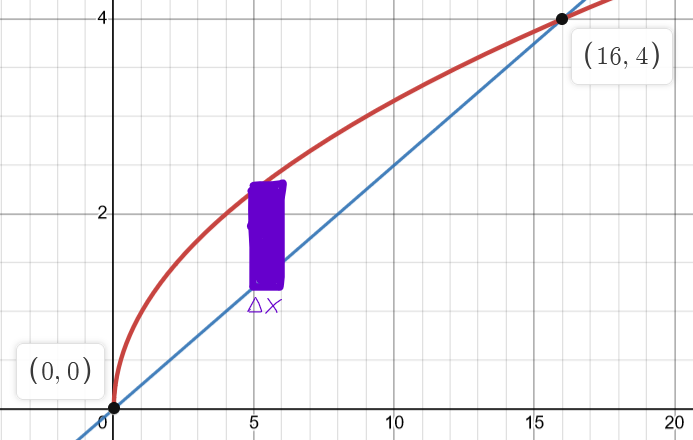
\includegraphics[width=0.6\textwidth]{images/6-1-2-a.png}
    
    \begin{red}
    The height of this slice is $\sqrt{x} - \tfrac14 x$, so the area of this slice is $(\sqrt{x} - \tfrac14 x)\Delta x$. Therefore, the area of this region is given by
    \[\int_{x=0}^{x=16} (\sqrt{x} - \tfrac14 x)\ dx. \]
    Wolfram$\mid$Alpha reports that the value of this integral is $\frac{32}{3}.$
    \end{red}
    \item The finite region bounded by $y=12-2x^2$ and $y=x^2-8$.
    
    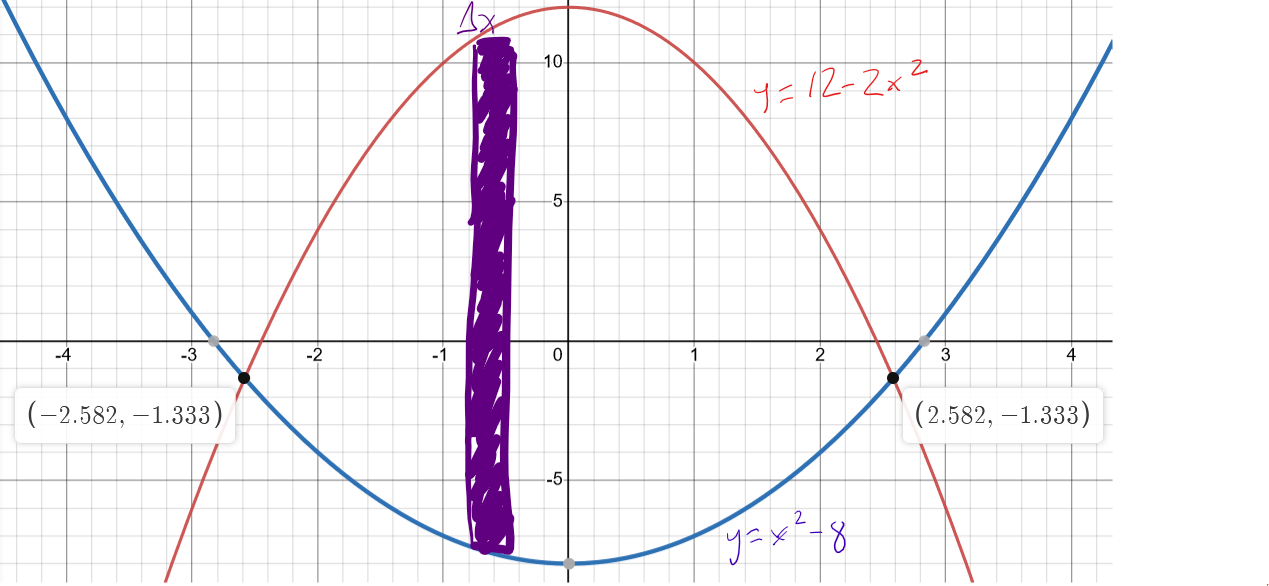
\includegraphics[width=0.6\textwidth]{images/6-1-2-b.png}
    
    \begin{red}
    The height of this slice is $(12-2x^2) - (x^2 - 8)$, so the area of this slice is $(20 - 3x^2)\Delta x$. Therefore, the area of this region is given by
    \[\int_{x=-2.582}^{x=2.582} (20 - 3x^2)\ dx. \]
    Wolfram$\mid$Alpha reports that the value of this integral is approximately $68.853$.
    \end{red}
    \item The area bounded by the $y$-axis, $f(x)=\cos(x)$, and $g(x)=\sin(x)$, where we consider the region formed by the first positive value of $x$ for which $f$ and $g$ intersect.
    
    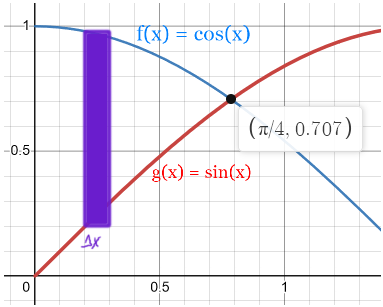
\includegraphics[width=0.6\textwidth]{images/6-1-2-c.png}
    
    \begin{red}
    The height of this slice is $\cos(x) - \sin(x)$, so the area of this slice is $(\cos(x) - \sin(x))\Delta x$. Therefore, the area of this region is given by
    \[\int_{x=0}^{x=\pi/4} (\cos(x) - \sin(x))\ dx. \]
    Wolfram$\mid$Alpha reports that the value of this integral is $\sqrt{2} - 1 \approx 0.414$.
    \end{red}
    \item The finite regions between the curves $y=x^3-x$ and $y=x^2$.
    
    \begin{minipage}{0.5\textwidth}
    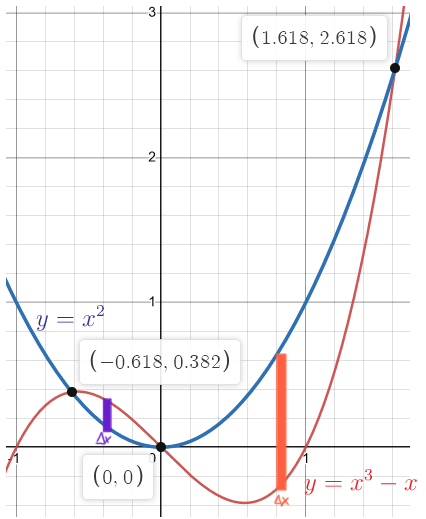
\includegraphics[width=\textwidth]{images/6-1-2-d.png}
    \end{minipage}
    \begin{minipage}{0.5\textwidth}
    \begin{red}
    I've drawn two representative slices because of how the functions cross over each other. 
    
    The height of the purple slice is $(x^3-x) - x^2$;
    
    the height of the orange slice is $x^2 - (x^3 - x)$.
    
    Therefore, the area of this region is given by
    \[\int_{x=-0.618}^{x=0} (x^3-x-x^2)\ dx + \int_{x=0}^{x=1.618}(x^2 - x^3 + x)\ dx. \]
    According to Wolfram$\mid$Alpha, the total area is approximately 1.0833.
    \end{red}
    \end{minipage}
\end{enumerate}

\pagebreak

\item (\href{https://faculty.gvsu.edu/boelkinm/Home/ACS/sec-6-1-area.html#ZJd}{AC Activity 6.1.3}) Our goal is to determine the area of the region described. \textbf{Note well}: At the step where you draw a representative slice, you need to make a choice about whether to slice vertically or horizontally.
\begin{enumerate}
    \item The finite region bounded by $x = y^2$ and $x = 6-2y^2$.
    
    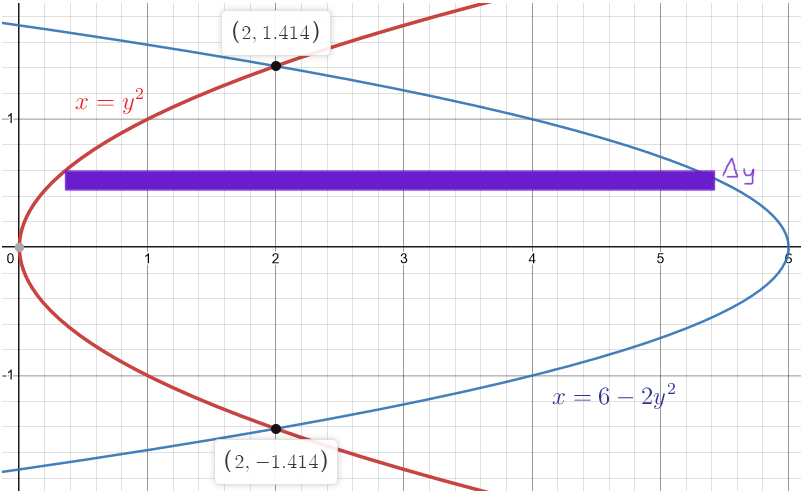
\includegraphics[width=0.6\textwidth]{images/6-1-3-a.png}
    
    \begin{red}
    A horizontal slice is certainly the way to go here. (There would be two species of vertical slices.) 
    
    The width of this slice is $(6-2y^2) - y^2$, so the area of this slice is $(6-3y^2)\Delta y$. So, the area of the region is 
    \[\int_{y=-1.414}^{y=1.414} (6-3y^2)\ dy. \]
    Wolfram$\mid$Alpha reports that the value of this integral is approximately $11.3137$.
    \end{red}
    \item The finite region bounded by $x = 1 - y^2$ and $x = 2 - 2y^2$.
    
    \begin{minipage}{0.5\textwidth}
    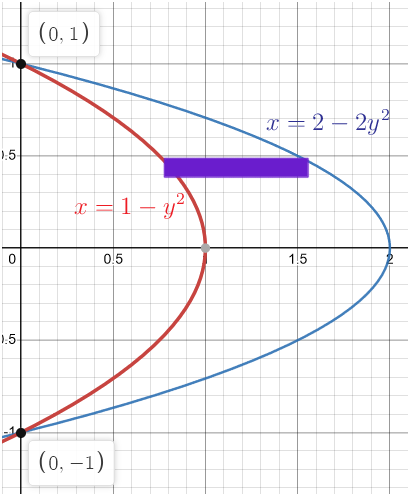
\includegraphics[width=\textwidth]{images/6-1-3-b.png}
    \end{minipage}
    \begin{minipage}{0.5\textwidth}
    \begin{red}
    (This region is clearly trying to be a shark, but I do not have the artistic merit to draw the picture it deserves.)
    
    Again, slicing horizontally is certainly the way to go. (Vertical slices would require \textbf{three} different species! \\ Do you see why?) 
    
    The width of the slice is $(2-2y^2) - (1-y^2)$, so the area of the slice is $(1-y^2) \Delta y$.
    
    Therefore, the area of this region is given by
    \[\int_{y=-1}^{y=1} (1-y^2)\ dy.\]
    According to Wolfram$\mid$Alpha, the total area is $\frac43$. (But this one's straightforward enough to do by hand.)
    \end{red}
    \end{minipage}
    
    \pagebreak
    
    \item The area bounded by the $x$-axis, $y=x^2$, and $y=2-x$.
    
    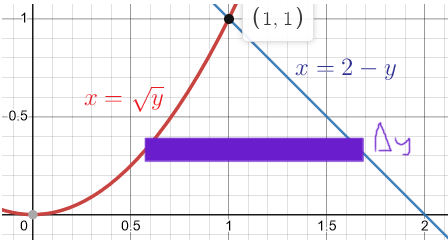
\includegraphics[width=0.7\textwidth]{images/6-1-3-c.png}
    
    \begin{red}
    A horizontal slice is the good choice here; vertical slices would produce two different species. We therefore have to solve for $x$ to write down the width.
    
    The width of the slice is $(2-y)-\sqrt{y}$, so the area of the slice is $(2-y-\sqrt{y}) \Delta y$.
    
    Therefore, the area of this region is given by
    \[\int_{y=0}^{y=1} (2-y-\sqrt{y})\ dy.\]
    According to Wolfram$\mid$Alpha, the total area is $\frac56$. (But this one's straightforward enough to do by hand.)
    \end{red}
    \item The finite region between the curves $x = y^2 - 2y$ and $y = x$.
    
    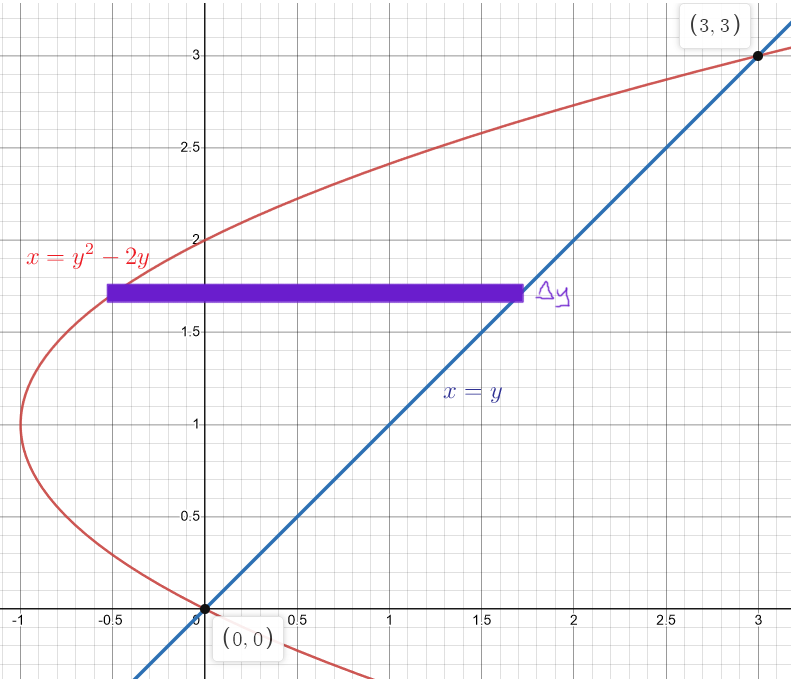
\includegraphics[width=0.6\textwidth]{images/6-1-3-d.png}
    
    \begin{red}
    A horizontal slice is certainly the way to go here. (There would be two species of vertical slices.) 
    
    The width of this slice is $y-(y^2-2y)$, so the area of this slice is $(3y-y^2)\Delta y$. Therefore, the area of this region is given by
    \[\int_{y=0}^{y=3} (3y-y^2)\ dy. \]
    Wolfram$\mid$Alpha reports that the value of this integral is $\frac92$ (straightforward to do by hand).
    \end{red}
\end{enumerate}

\end{enumerate}
\end{document}